\chapter{Experiments and results}
\label{AER}

\section{What Does A Good Curve Look Like?}
Assuming a very simple model, with no washin or washout rate, a good bacteria growth curve would look like a mountain, with a clear rise, peak, and fall in population levels. 
For a given initial condition, the bacteria start to consume resources and replicate leading to exponential growth. 
The phages start to infect the bacteria and eventually the bacteria start to die, releasing new phages. 
The new phages infect more bacteria, putting pressure on the bacteria growth. 
Eventually, more bacteria are being infected than being created, causing the decline in bacteria population. 
\Cref{fig:created:a_good_curve_linear} shows an example of a good curve. 
\Cref{fig:created:a_good_curve_logarithmic} is the same plot but with a logarithmic y-axis. 

As the bacteria population grow, the resource consumption speeds up until there are trace amount of resources left at $t=8$. 
The uninfected and infected bacteria exhibit exponential growth, peaking at 1617 at $t=3.99$ and 3463 at $t=5.27$ respectively. 
The delay in the uninfected to infected bacteria's peak is due to the infection stages and latent period of the phage infection. 
The bacteria sum do not have as stark of a peak in comparison to the uninfected and infected bacteria, due to the graph measuring all bacteria populations, but the peak of 3805 at $t=4.89$ is still clear. 
The phages saw a significant increase in population count at around $t=4$, coinciding with the peak in uninfected bacteria. 
At this point in time, the infection rate is larger than the bacteria replication rate, so the bacteria are starting to die out even though there are still sufficient resources remaining. 
At around $t=4$ is when the the resource consumption rate inflects. 
The rate at which the resources are being consumed starts to slow down, showing a decreasing sigmoid shape. 
The total bacteria population reached a peak of 3805 at $t=4.89$, a 76.1x increase in population count from the initial 50 starting uninfected bacteria. 
The phage population reached a peak of 2584 phages at $t=15$, a 258.4x increase in population count. 

\begin{figure}[h!]
    \centering
    \begin{subfigure}{1\linewidth}
        \centering
        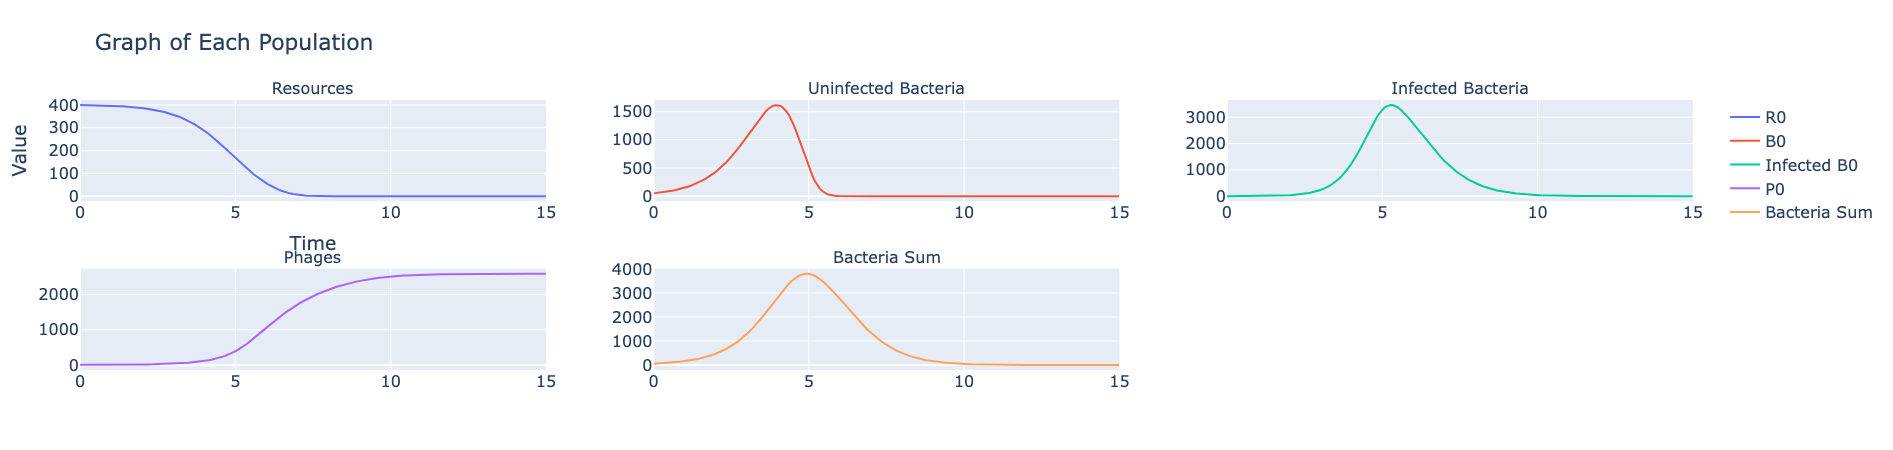
\includegraphics[width=\linewidth]{Plots/Created/a_good_curve_linear.png}
        \caption{
            Linear y-axis for a "good" plot. 
        }
        \label{fig:created:a_good_curve_linear}
    \end{subfigure}
    \hfill
    \begin{subfigure}{1\linewidth}
        \centering
        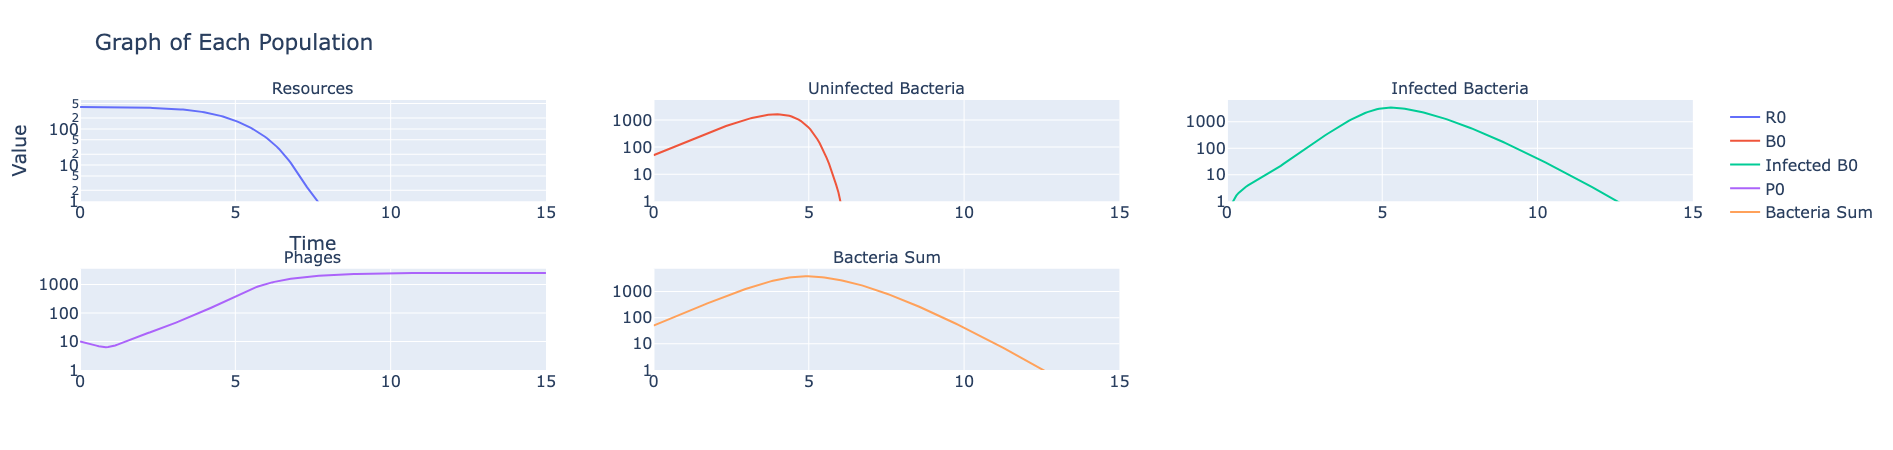
\includegraphics[width=\linewidth]{Plots/Created/a_good_curve_logarithmic.png}
        \caption{
            Logarithmic y-axis for a "good" plot. 
        }
        \label{fig:created:a_good_curve_logarithmic}
    \end{subfigure}
    \label{fig:created:a_good_curve}
    \caption{The parameters used for this plot can be found in \Cref{tab:appendixE:a_good_curve}}
\end{figure}



\section{SOBOL Sensitivity Analysis}
With any model, it is important to understand how a change in parameter value affects the change in output. 
Some models will have parameters that are more important and affect the model output more than other parameters. 
A SOBOL analysis was run on the golden model for three different analyses. 
\Cref{fig:created:SOBOL_average} shows the impact that the parameter had on the final value of the population at $t=15$. 
\Cref{fig:created:SOBOL_average} and \Cref{fig:created:SOBOL_variance} likewise show the impact that the parameters had on the average value and variance of the population throughout the simulation respectively. 
The parameters that were tested include all the parameters listed in the extended golden model, except for $M$. 
$M$, the number of stages that the infection goes through, can not be tested as $M$ hardcodes the number of infection stages that the bacteria has to go through. 
The hardcoding is done before the simulation framework starts. As such, it is not possible to change $M$. 

The first thing that can be noticed is how the bar plots across the final value, average, and variance analyses have very similar values. 

\begin{figure}
    \centering
    \begin{subfigure}{0.49\linewidth}
        \centering
        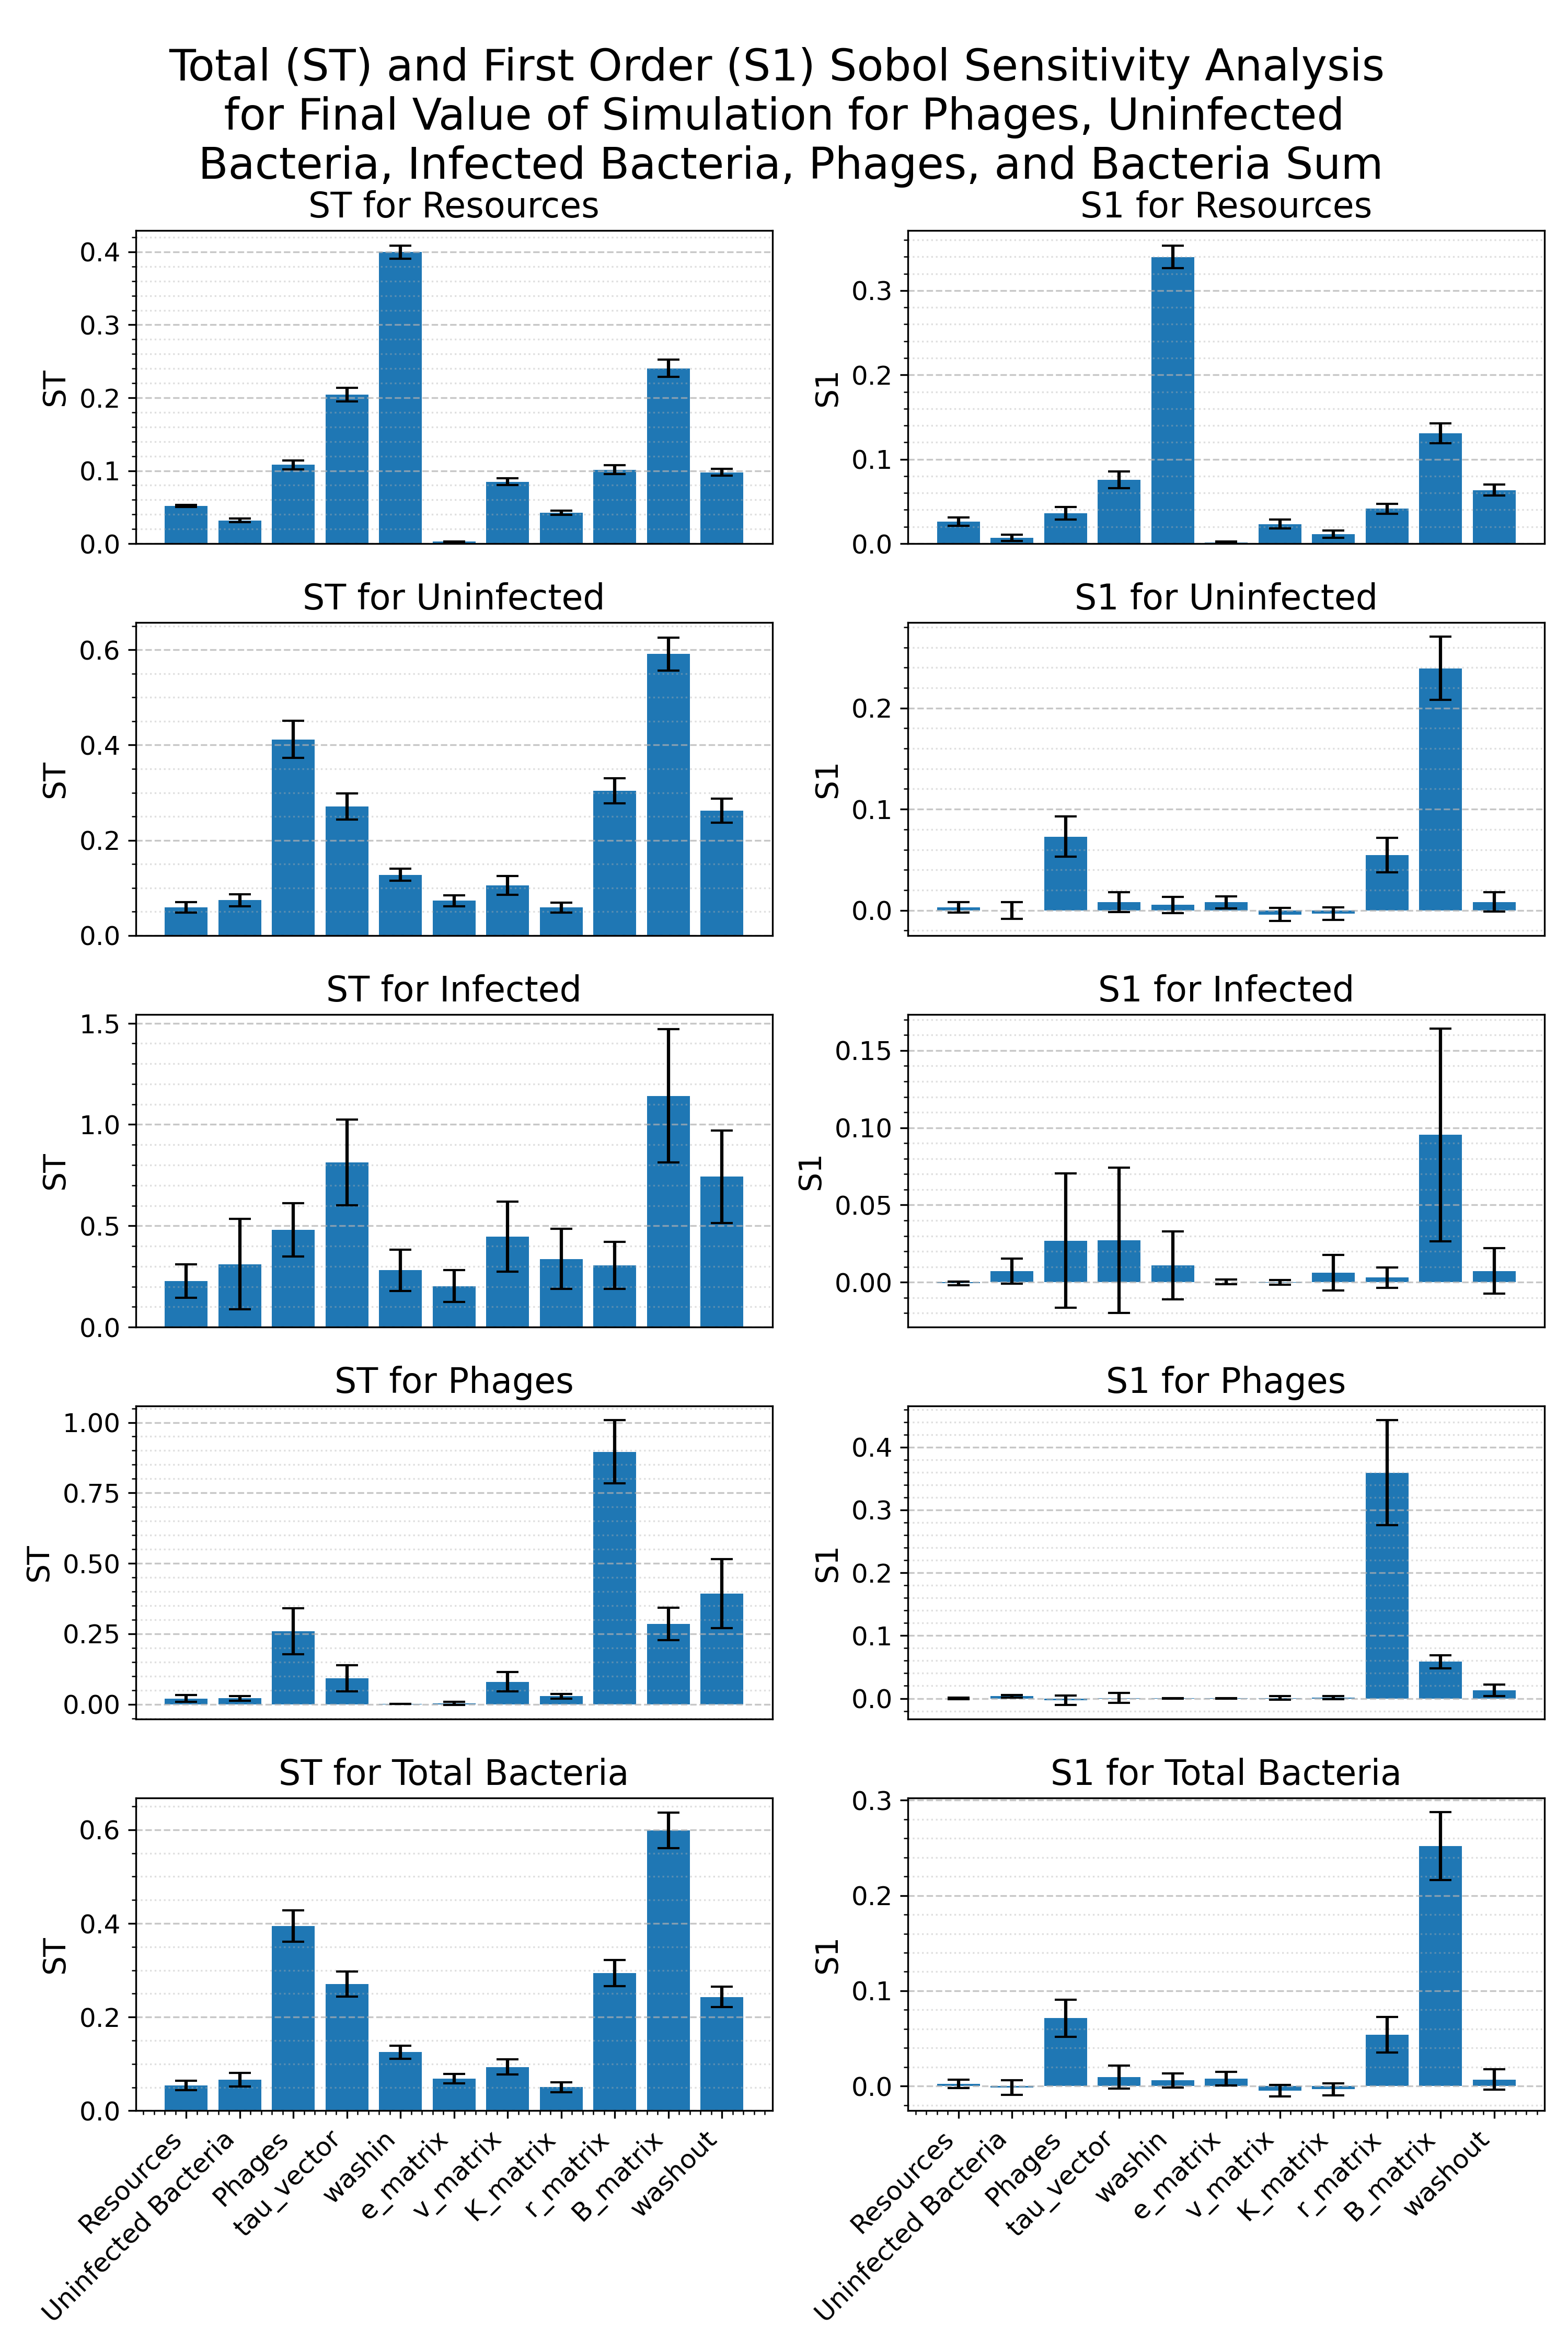
\includegraphics[width=\linewidth]{Plots/Created/SOBOL_analysis_1747923579_Final.png}
        \caption{
            The total and first order sensitivity for the golden model for the final Resource, Uninfected, Infected, Phage, and Total Bacteria population value. 
        }
        \label{fig:created:SOBOL_final}
    \end{subfigure}
    \hfill
    \begin{subfigure}{0.49\linewidth}
        \centering
        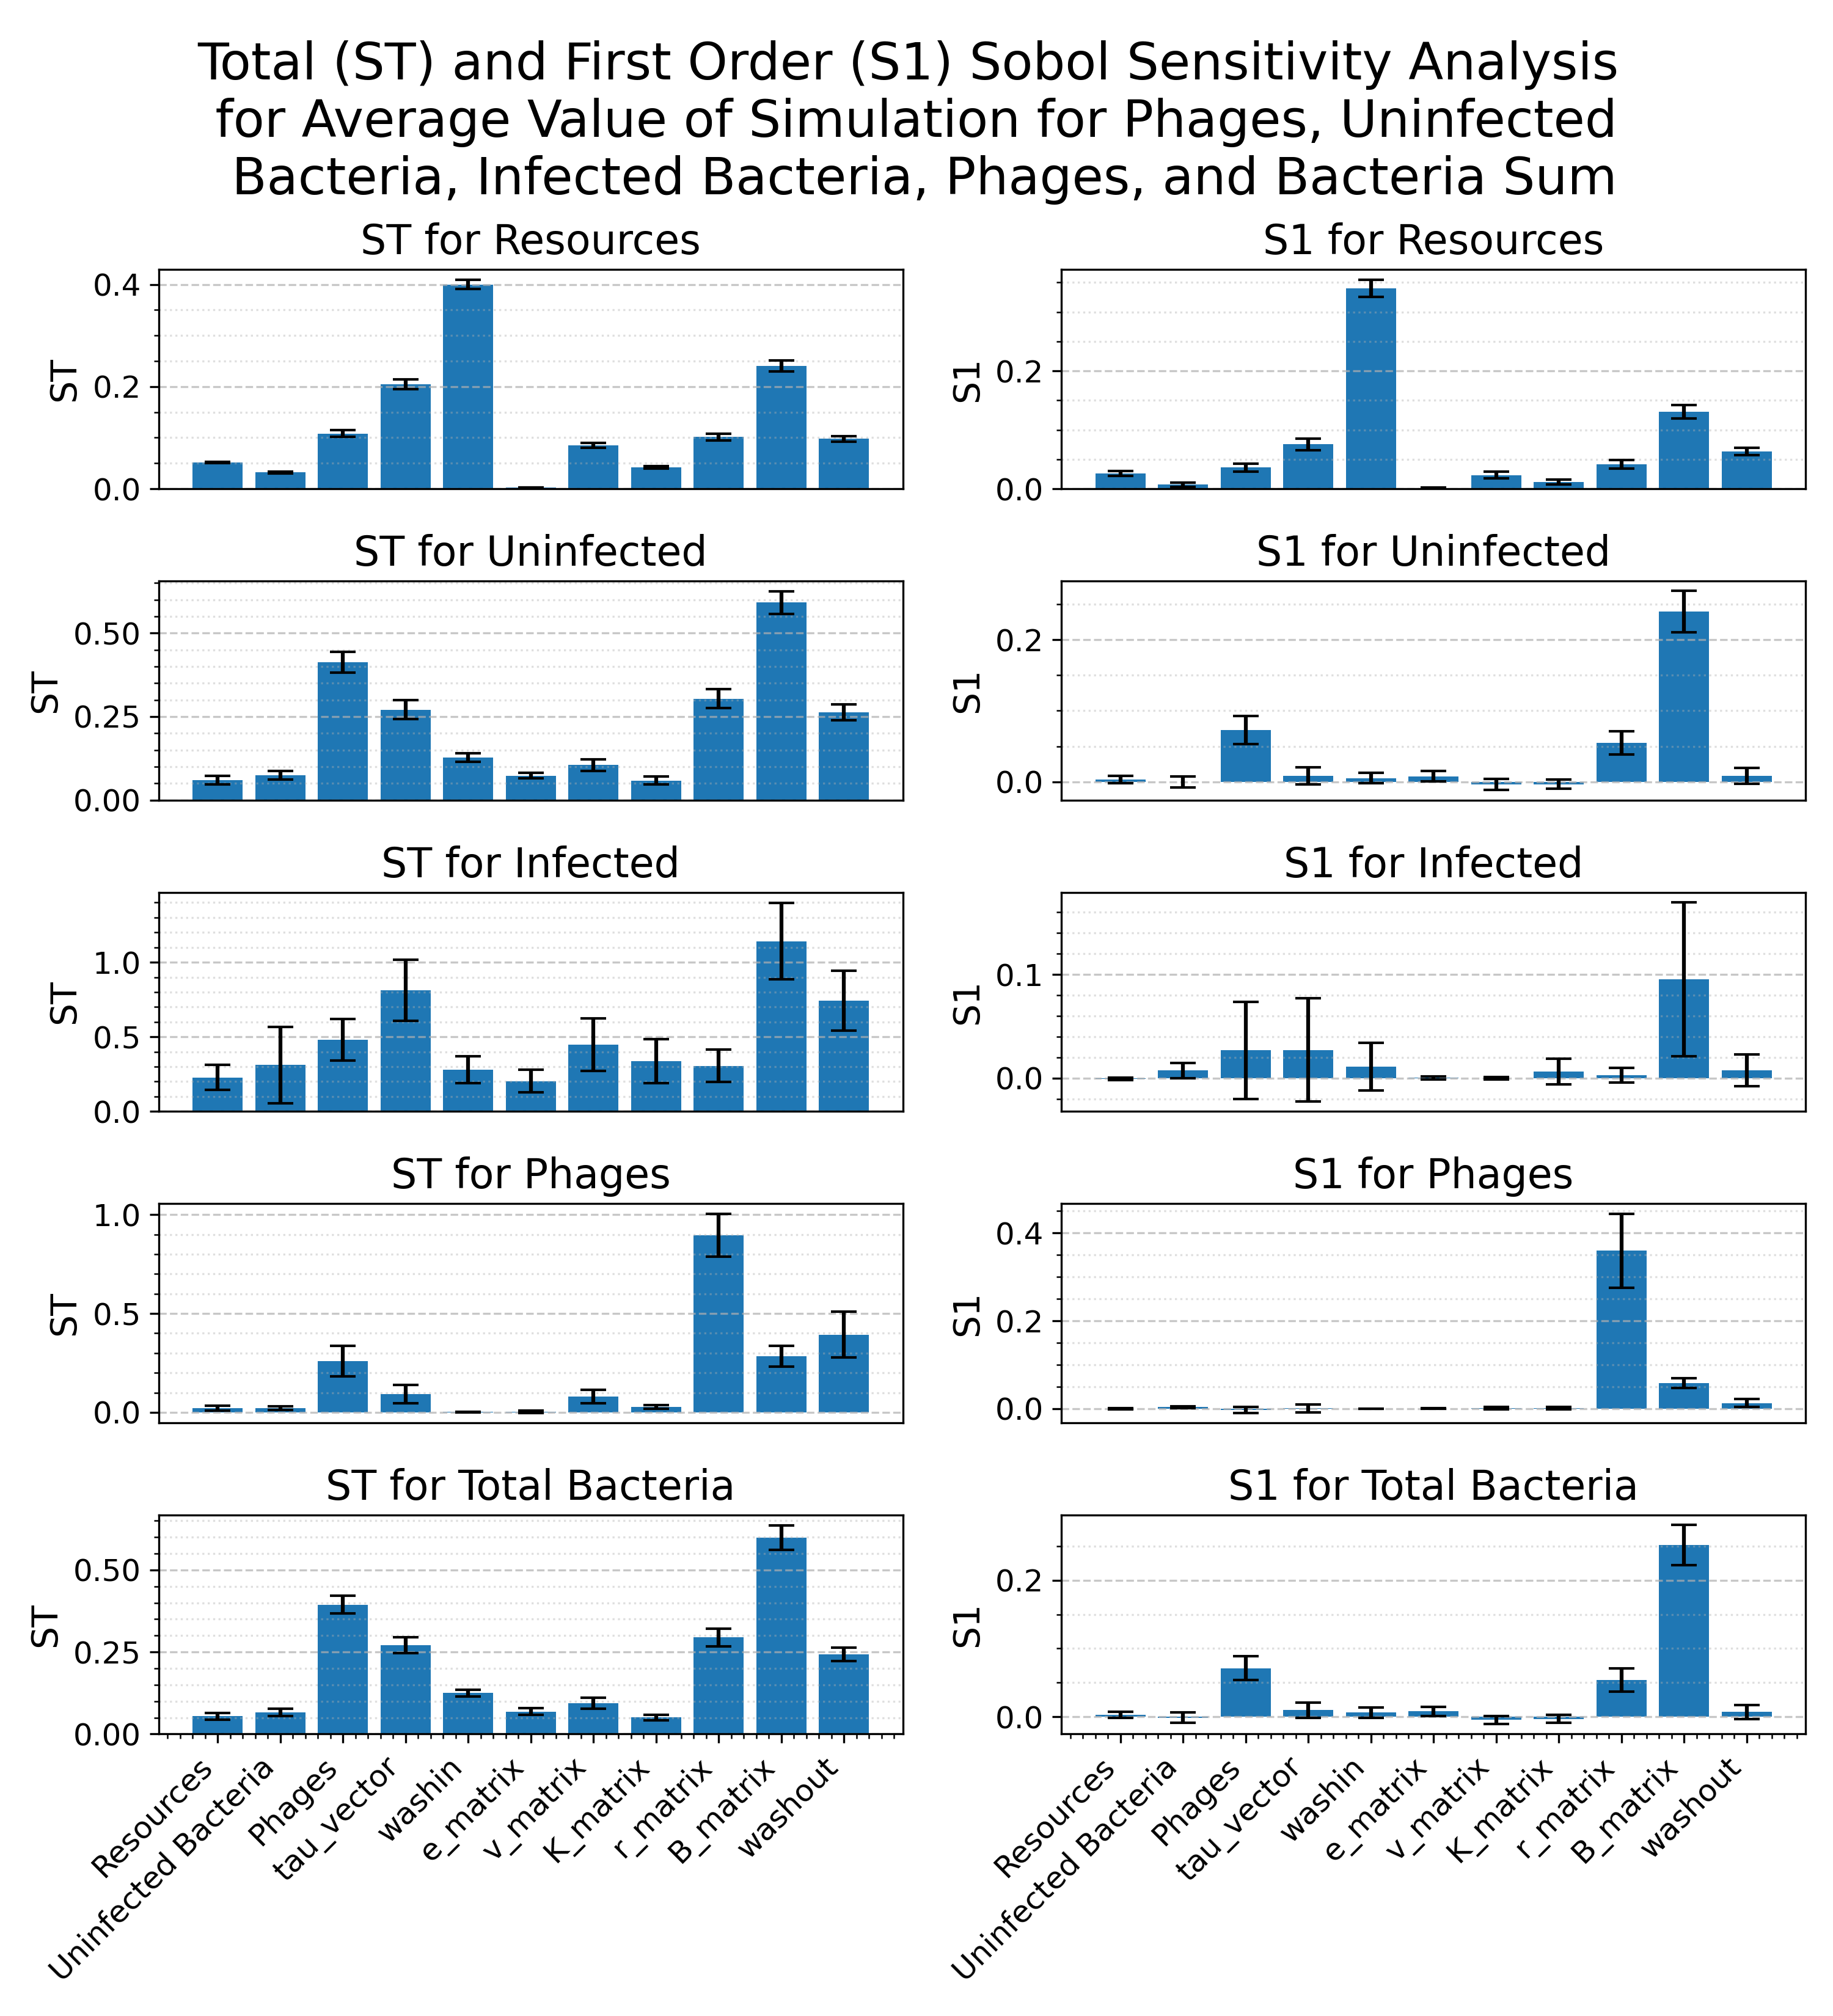
\includegraphics[width=\linewidth]{Plots/Created/SOBOL_analysis_1747923579_Average.png}
        \caption{
            The total and first order sensitivity for the golden model for the average Resource, Uninfected, Infected, Phage, and Total Bacteria population value. 
        }
        \label{fig:created:SOBOL_average}
    \end{subfigure}
    \hfill
    \begin{subfigure}{0.49\linewidth}
        \centering
        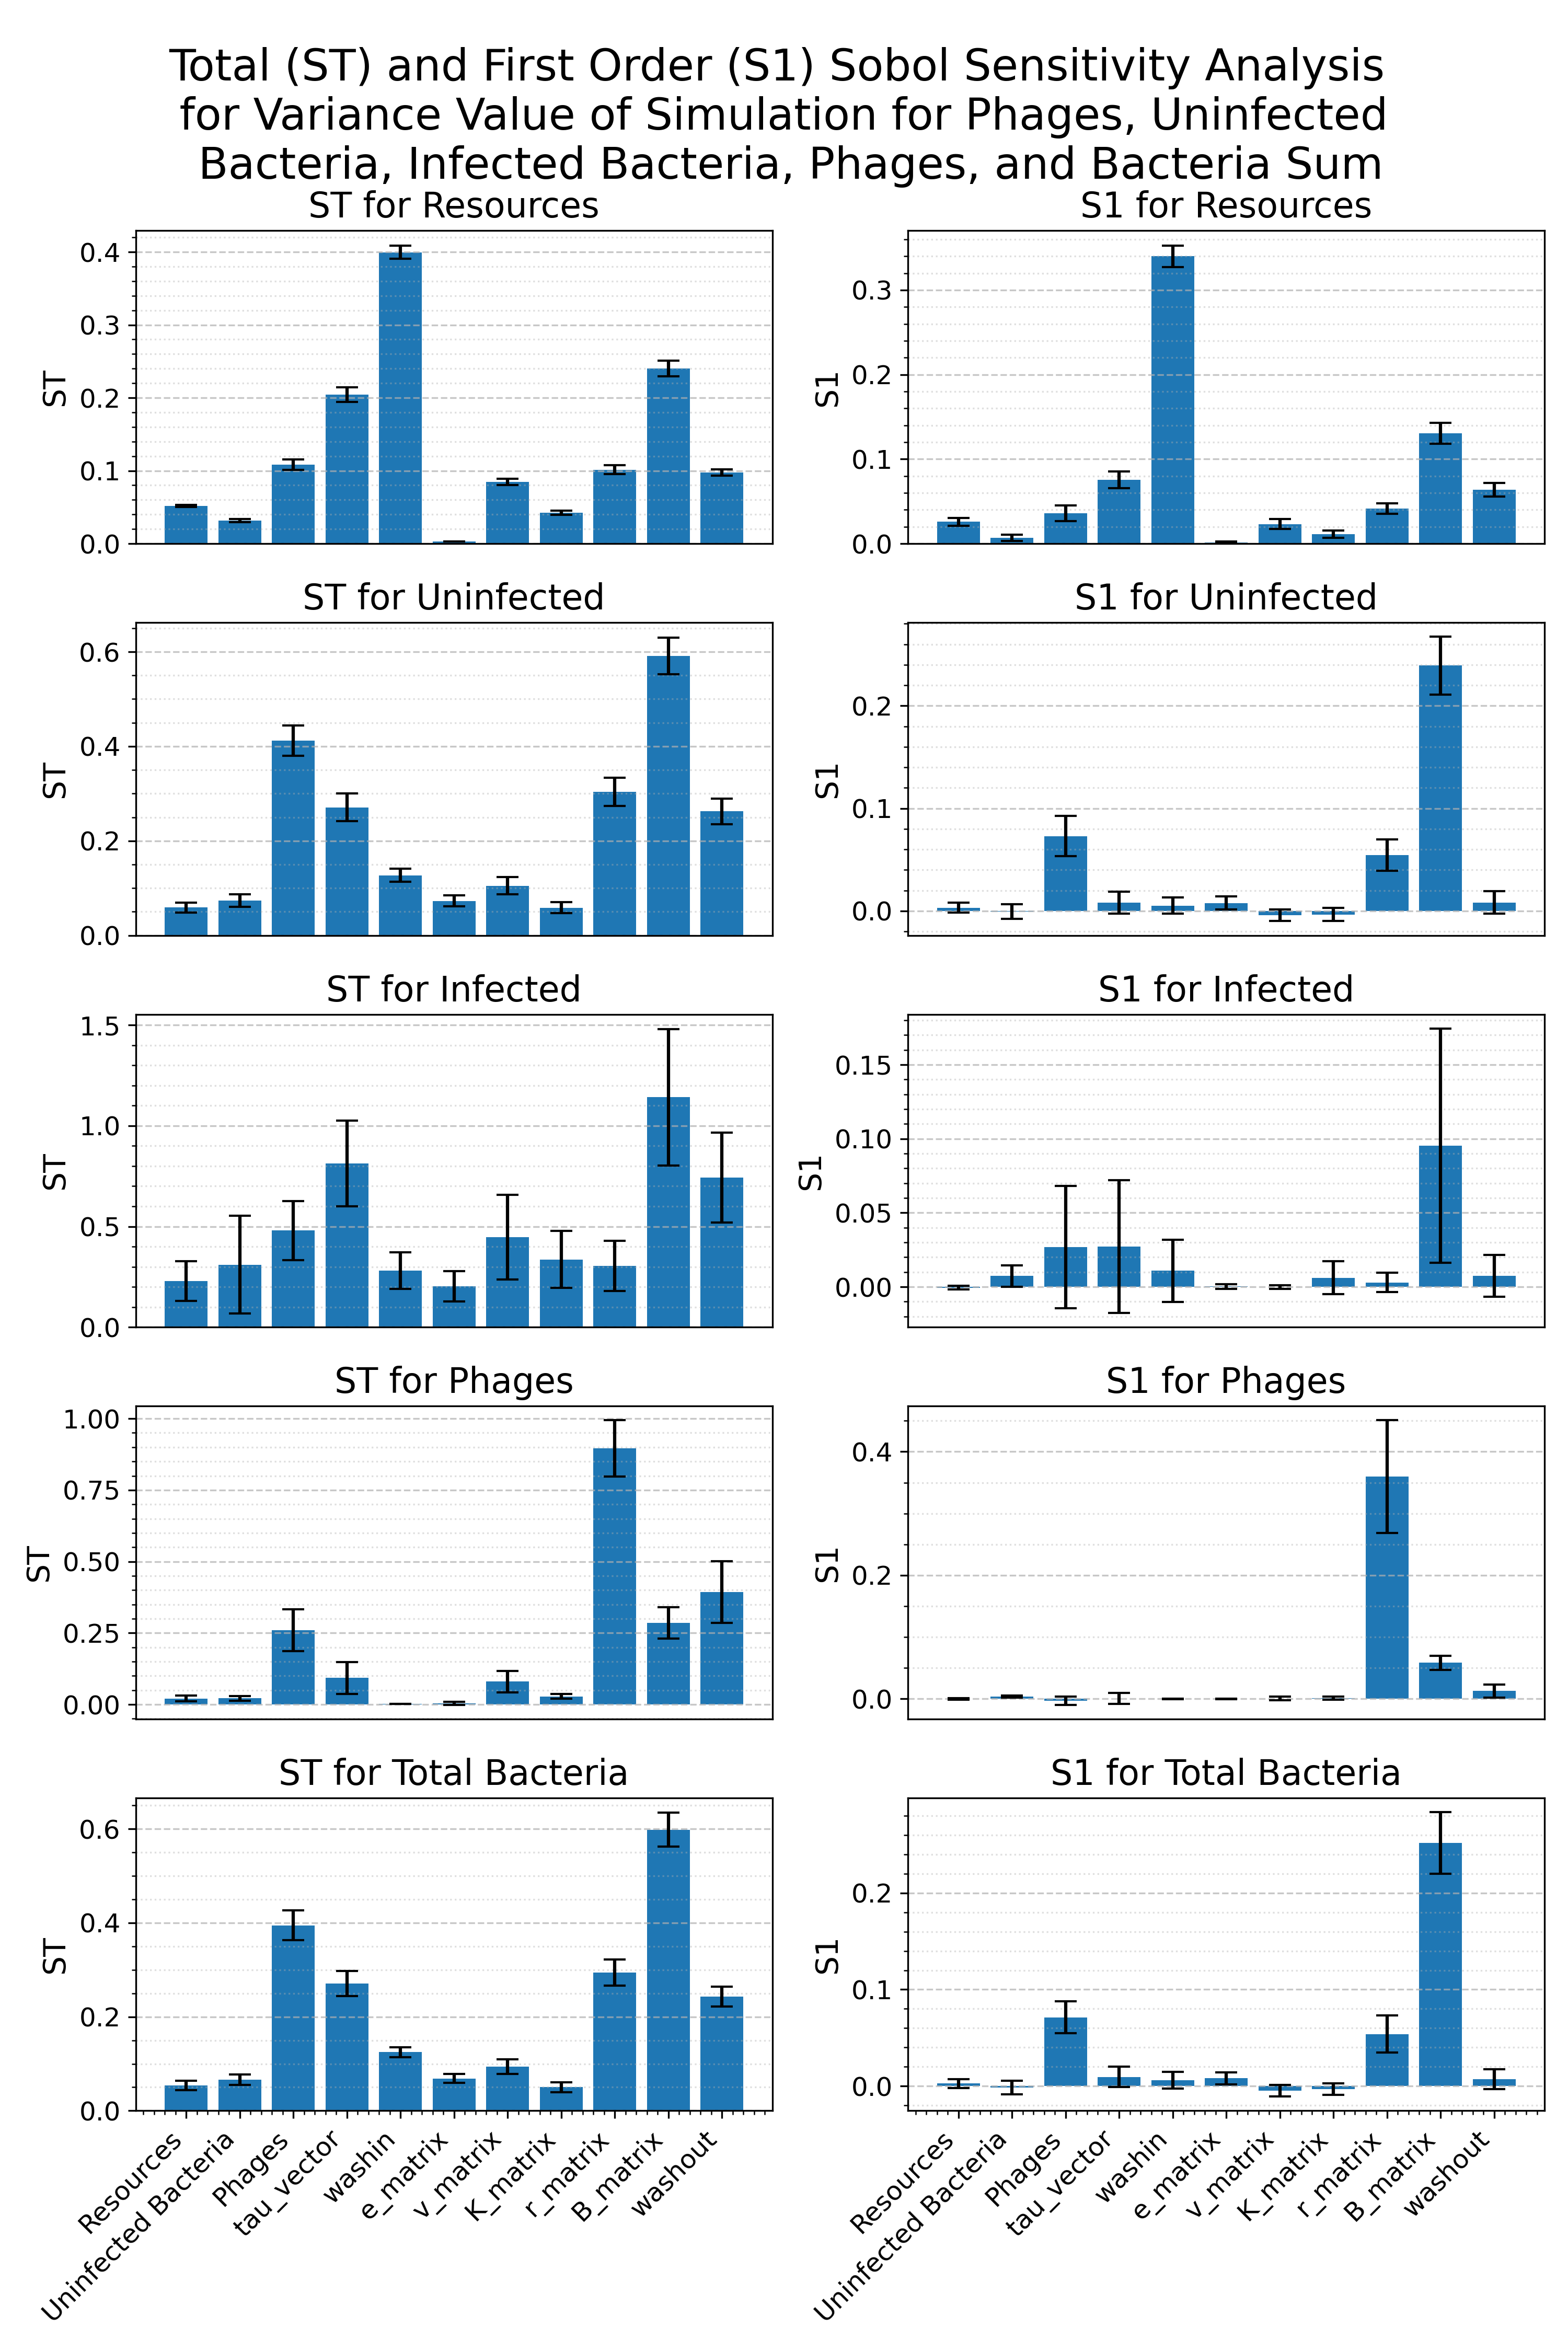
\includegraphics[width=\linewidth]{Plots/Created/SOBOL_analysis_1747923579_Variance.png}
        \caption{
            The total and first order sensitivity for the golden model for the variance of Resource, Uninfected, Infected, Phage, and Total Bacteria value. 
        }
        \label{fig:created:SOBOL_variance}
    \end{subfigure}
    \caption{The SOBOL analysis for the simple $1\times 1 \times 1$ golden model. }
\end{figure}
